% Options for packages loaded elsewhere
\PassOptionsToPackage{unicode}{hyperref}
\PassOptionsToPackage{hyphens}{url}
\PassOptionsToPackage{dvipsnames,svgnames,x11names}{xcolor}
%
\documentclass[
  ignorenonframetext,
  aspectratio=169,
]{beamer}
\usepackage{pgfpages}
\setbeamertemplate{caption}[numbered]
\setbeamertemplate{caption label separator}{: }
\setbeamercolor{caption name}{fg=normal text.fg}
\beamertemplatenavigationsymbolshorizontal
% Prevent slide breaks in the middle of a paragraph
\widowpenalties 1 10000
\raggedbottom
\setbeamertemplate{part page}{
  \centering
  \begin{beamercolorbox}[sep=16pt,center]{part title}
    \usebeamerfont{part title}\insertpart\par
  \end{beamercolorbox}
}
\setbeamertemplate{section page}{
  \centering
  \begin{beamercolorbox}[sep=12pt,center]{part title}
    \usebeamerfont{section title}\insertsection\par
  \end{beamercolorbox}
}
\setbeamertemplate{subsection page}{
  \centering
  \begin{beamercolorbox}[sep=8pt,center]{part title}
    \usebeamerfont{subsection title}\insertsubsection\par
  \end{beamercolorbox}
}
\AtBeginPart{
  \frame{\partpage}
}
\AtBeginSection{
  \ifbibliography
  \else
    \frame{\sectionpage}
  \fi
}
\AtBeginSubsection{
  \frame{\subsectionpage}
}

\usepackage{amsmath,amssymb}
\usepackage{iftex}
\ifPDFTeX
  \usepackage[T1]{fontenc}
  \usepackage[utf8]{inputenc}
  \usepackage{textcomp} % provide euro and other symbols
\else % if luatex or xetex
  \usepackage{unicode-math}
  \defaultfontfeatures{Scale=MatchLowercase}
  \defaultfontfeatures[\rmfamily]{Ligatures=TeX,Scale=1}
\fi
\usetheme[]{Hannover}
\usecolortheme{rose}
\usepackage[]{libertinus}
\ifPDFTeX\else  
    % xetex/luatex font selection
\fi
% Use upquote if available, for straight quotes in verbatim environments
\IfFileExists{upquote.sty}{\usepackage{upquote}}{}
\IfFileExists{microtype.sty}{% use microtype if available
  \usepackage[]{microtype}
  \UseMicrotypeSet[protrusion]{basicmath} % disable protrusion for tt fonts
}{}
\makeatletter
\@ifundefined{KOMAClassName}{% if non-KOMA class
  \IfFileExists{parskip.sty}{%
    \usepackage{parskip}
  }{% else
    \setlength{\parindent}{0pt}
    \setlength{\parskip}{6pt plus 2pt minus 1pt}}
}{% if KOMA class
  \KOMAoptions{parskip=half}}
\makeatother
\usepackage{xcolor}
\newif\ifbibliography
\setlength{\emergencystretch}{3em} % prevent overfull lines
\setcounter{secnumdepth}{-\maxdimen} % remove section numbering


\providecommand{\tightlist}{%
  \setlength{\itemsep}{0pt}\setlength{\parskip}{0pt}}\usepackage{longtable,booktabs,array}
\usepackage{calc} % for calculating minipage widths
\usepackage{caption}
% Make caption package work with longtable
\makeatletter
\def\fnum@table{\tablename~\thetable}
\makeatother
\usepackage{graphicx}
\makeatletter
\def\maxwidth{\ifdim\Gin@nat@width>\linewidth\linewidth\else\Gin@nat@width\fi}
\def\maxheight{\ifdim\Gin@nat@height>\textheight\textheight\else\Gin@nat@height\fi}
\makeatother
% Scale images if necessary, so that they will not overflow the page
% margins by default, and it is still possible to overwrite the defaults
% using explicit options in \includegraphics[width, height, ...]{}
\setkeys{Gin}{width=\maxwidth,height=\maxheight,keepaspectratio}
% Set default figure placement to htbp
\makeatletter
\def\fps@figure{htbp}
\makeatother
% definitions for citeproc citations
\NewDocumentCommand\citeproctext{}{}
\NewDocumentCommand\citeproc{mm}{%
  \begingroup\def\citeproctext{#2}\cite{#1}\endgroup}
\makeatletter
 % allow citations to break across lines
 \let\@cite@ofmt\@firstofone
 % avoid brackets around text for \cite:
 \def\@biblabel#1{}
 \def\@cite#1#2{{#1\if@tempswa , #2\fi}}
\makeatother
\newlength{\cslhangindent}
\setlength{\cslhangindent}{1.5em}
\newlength{\csllabelwidth}
\setlength{\csllabelwidth}{3em}
\newenvironment{CSLReferences}[2] % #1 hanging-indent, #2 entry-spacing
 {\begin{list}{}{%
  \setlength{\itemindent}{0pt}
  \setlength{\leftmargin}{0pt}
  \setlength{\parsep}{0pt}
  % turn on hanging indent if param 1 is 1
  \ifodd #1
   \setlength{\leftmargin}{\cslhangindent}
   \setlength{\itemindent}{-1\cslhangindent}
  \fi
  % set entry spacing
  \setlength{\itemsep}{#2\baselineskip}}}
 {\end{list}}
\usepackage{calc}
\newcommand{\CSLBlock}[1]{\hfill\break\parbox[t]{\linewidth}{\strut\ignorespaces#1\strut}}
\newcommand{\CSLLeftMargin}[1]{\parbox[t]{\csllabelwidth}{\strut#1\strut}}
\newcommand{\CSLRightInline}[1]{\parbox[t]{\linewidth - \csllabelwidth}{\strut#1\strut}}
\newcommand{\CSLIndent}[1]{\hspace{\cslhangindent}#1}

\makeatletter
\@ifpackageloaded{caption}{}{\usepackage{caption}}
\AtBeginDocument{%
\ifdefined\contentsname
  \renewcommand*\contentsname{Table of contents}
\else
  \newcommand\contentsname{Table of contents}
\fi
\ifdefined\listfigurename
  \renewcommand*\listfigurename{List of Figures}
\else
  \newcommand\listfigurename{List of Figures}
\fi
\ifdefined\listtablename
  \renewcommand*\listtablename{List of Tables}
\else
  \newcommand\listtablename{List of Tables}
\fi
\ifdefined\figurename
  \renewcommand*\figurename{Figure}
\else
  \newcommand\figurename{Figure}
\fi
\ifdefined\tablename
  \renewcommand*\tablename{Table}
\else
  \newcommand\tablename{Table}
\fi
}
\@ifpackageloaded{float}{}{\usepackage{float}}
\floatstyle{ruled}
\@ifundefined{c@chapter}{\newfloat{codelisting}{h}{lop}}{\newfloat{codelisting}{h}{lop}[chapter]}
\floatname{codelisting}{Listing}
\newcommand*\listoflistings{\listof{codelisting}{List of Listings}}
\makeatother
\makeatletter
\makeatother
\makeatletter
\@ifpackageloaded{caption}{}{\usepackage{caption}}
\@ifpackageloaded{subcaption}{}{\usepackage{subcaption}}
\makeatother
\ifLuaTeX
  \usepackage{selnolig}  % disable illegal ligatures
\fi
\usepackage{bookmark}

\IfFileExists{xurl.sty}{\usepackage{xurl}}{} % add URL line breaks if available
\urlstyle{same} % disable monospaced font for URLs
\hypersetup{
  pdftitle={Longitudinal Design},
  pdfauthor={Usman Afzali, PhD},
  colorlinks=true,
  linkcolor={Maroon},
  filecolor={Maroon},
  citecolor={Blue},
  urlcolor={Blue},
  pdfcreator={LaTeX via pandoc}}

\title{Longitudinal Design}
\author{Usman Afzali, PhD}
\date{2024-10-07}
\logo{
\includegraphics{mds.png}}

\begin{document}
\frame{\titlepage}

\begin{frame}
\begin{figure}

\begin{minipage}{\linewidth}
\begin{center}

\includegraphics[width=0.5\textwidth,height=\textheight]{figs/mds.png}
\end{center}

\includegraphics{figs/sponsors.png}\end{minipage}%

\end{figure}%
\end{frame}

\begin{frame}{Outline}
\phantomsection\label{outline}
\begin{itemize}
\tightlist
\item
  Social perspective
\item
  Developmental perspective
\item
  Identity denial
\item
  Negative consequences
\item
  What to do?
\end{itemize}
\end{frame}

\begin{frame}
\textbf{Longitudinal Design}

\begin{itemize}[<+->]
\tightlist
\item
  Measuring a variable (or variables) in the same group of subjects over
  a period of time.
\item
  Subjects are generally in the same cohort and they age together.
\item
  It is a within-subjects design (pretest-posttest)
\end{itemize}
\end{frame}

\begin{frame}
Example: Measuring IQ at 40, 60, and 80 years of age in the same cohort
(or even the same individuals).

\begin{center}
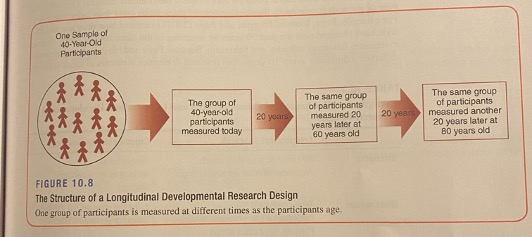
\includegraphics{figs/iq.jpg}
\end{center}
\end{frame}

\begin{frame}{Social experiment}
\phantomsection\label{social-experiment}
\begin{columns}[c,totalwidth=8em]
\begin{column}{0.4\textwidth}
\begin{itemize}[<+->]
\tightlist
\item
  \textbf{Task 1}: Estimate the number of dots on each slide
\item
  \textbf{Outcome}: \emph{``Over-estimators''} and
  \emph{``under-estimators''}
\item
  Divided into two random groups
\item
  \textbf{Task 2}: Allocate points to other participants that can be
  cashed for money.
\end{itemize}
\end{column}

\begin{column}{0.6\textwidth}
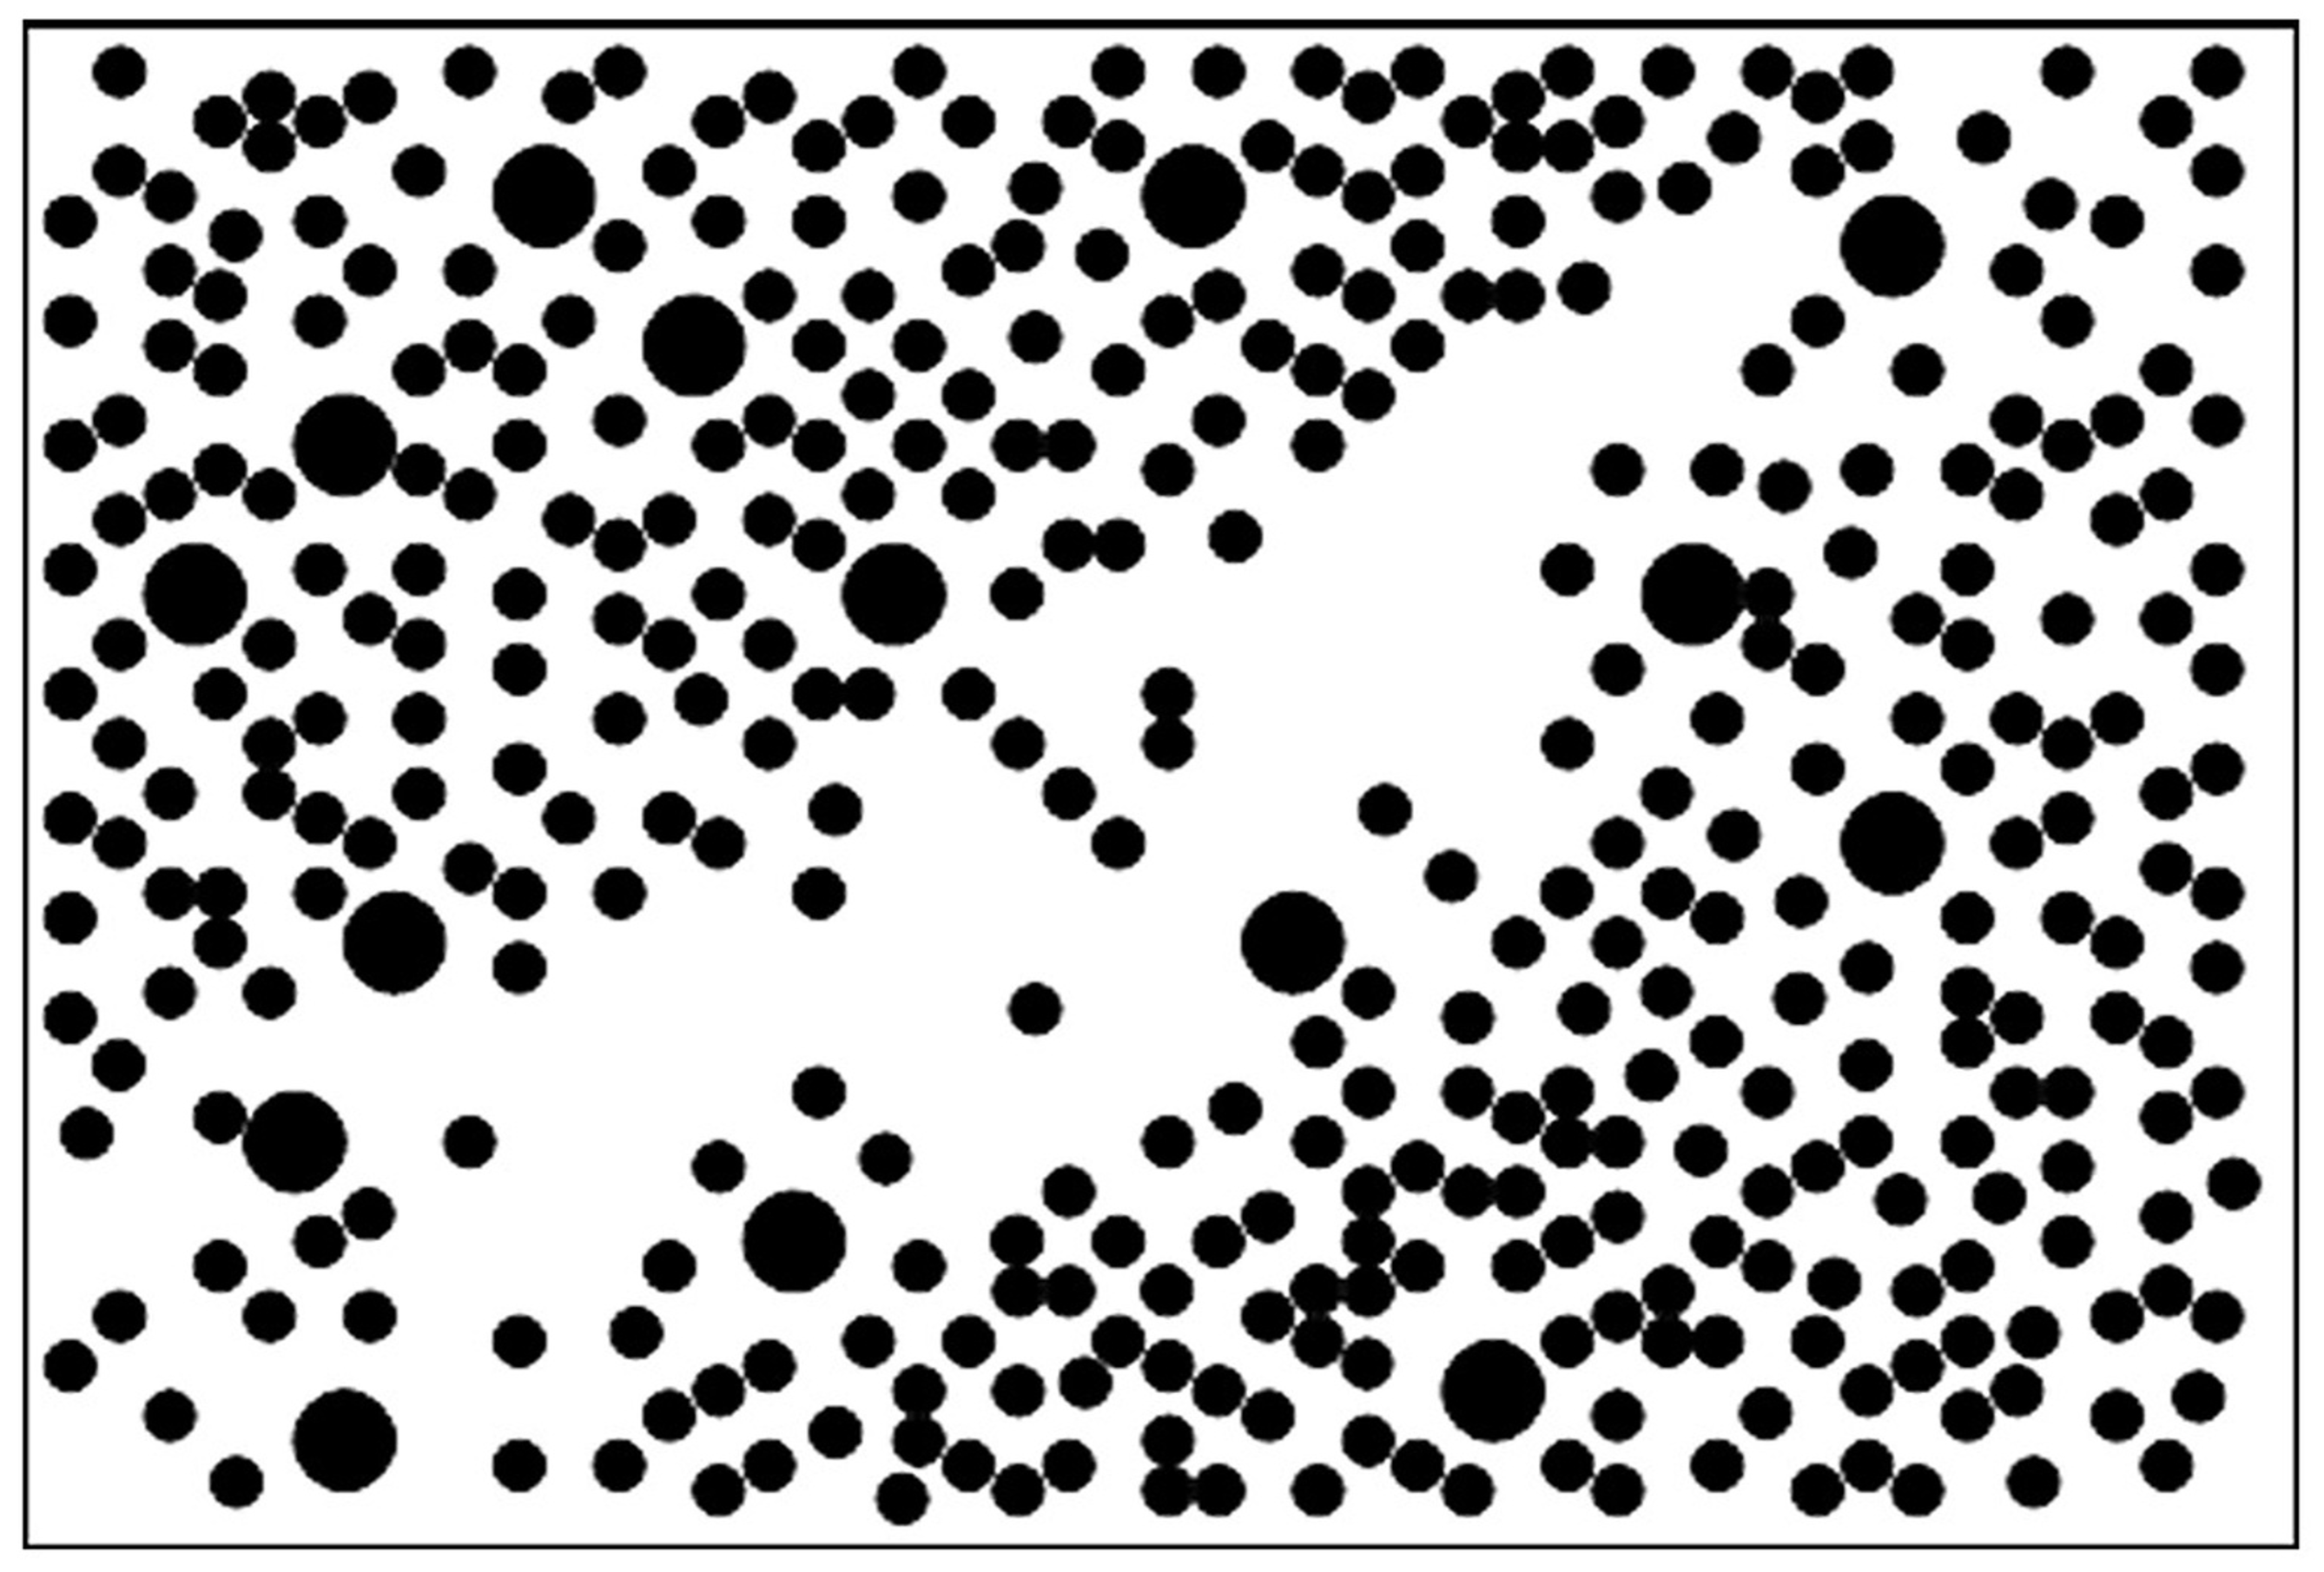
\includegraphics{figs/tajfel.png}
\end{column}
\end{columns}
\end{frame}

\begin{frame}{Strengths and Weaknesses}
\phantomsection\label{strengths-and-weaknesses}
\begin{itemize}[<+->]
\tightlist
\item
  The absence of cohort effect
\item
  Allows studies changes of behaviour in individuals across time
\item
  Time consuming (for researchers and subjects), needs commitment
\item
  Very expensive
\item
  High drop-out rates (aka sample/participant attrition), that weakens
  internal validity (how?)
\end{itemize}
\end{frame}

\begin{frame}{The need for self-esteem}
\phantomsection\label{the-need-for-self-esteem}
Kassin et al.~(2021)

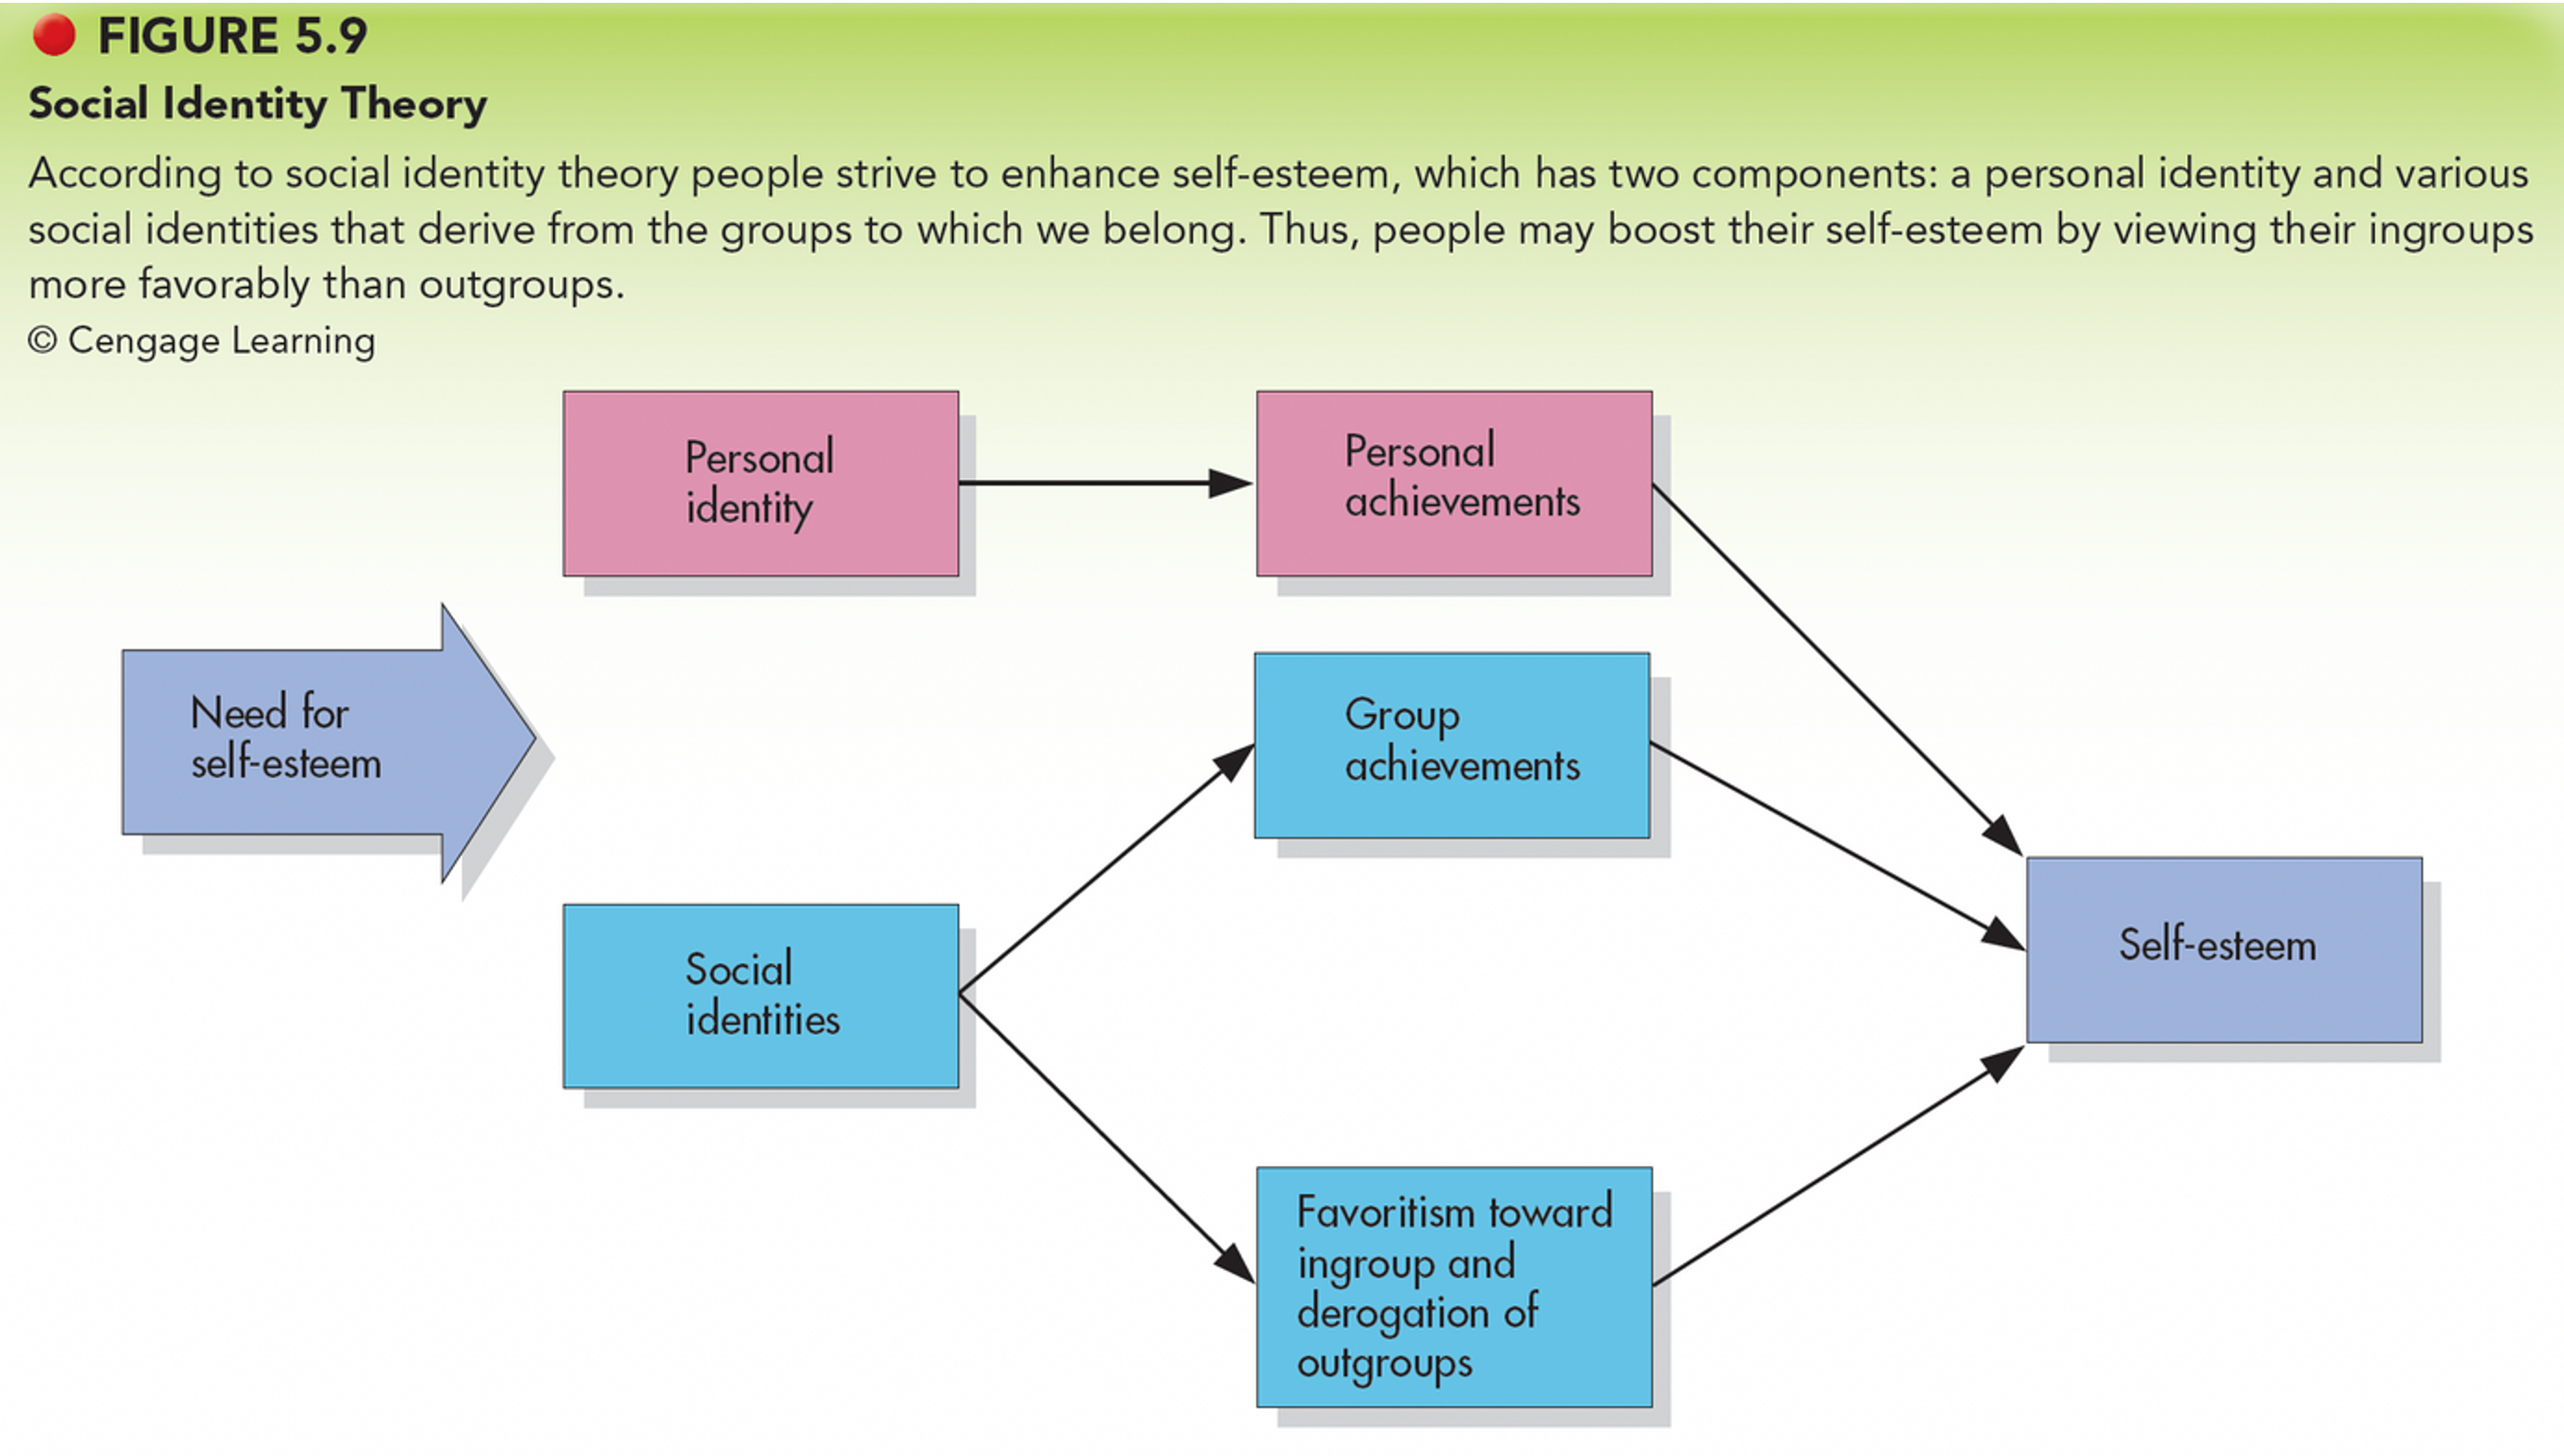
\includegraphics[width=0.9\textwidth,height=\textheight]{figs/selfesteem.png}
\end{frame}

\begin{frame}
\begin{itemize}[<+->]
\tightlist
\item
  \textbf{Advantage}: Derive pride from our connections
\item
  \textbf{Disadvantage}: The need to belittle \emph{``them''} in order
  to feel secure about \emph{``us''}.
\item
  Examples: Religious fervor, racial and ethnic conceit, aggressive
  nationalism, and even gossiping (Bosson et al. 2006; Weaver and Bosson
  2011)
\item
  When people shared negative attitudes about a third party, they felt
  closer to each other.
\end{itemize}
\end{frame}

\begin{frame}{ADesign and Analysis Considerations}
\phantomsection\label{adesign-and-analysis-considerations}
\begin{itemize}[<+->]
\tightlist
\item
  Representative sampling
\item
  Minimizing selection bias
\item
  Choosing appropriate measurement tools
\item
  Combining quantitative and qualitative approaches
\item
  Analysing growth trajectories (e.g., growth curve modelling)
\item
  Exploring inter-individual and intra-individual differences
\end{itemize}
\end{frame}

\begin{frame}
\begin{itemize}[<+->]
\tightlist
\item
  For example, this person might start expressing or endorsing negative
  stereotypes about Muslims, such as portraying them as
  \emph{terrorists}, \emph{backward}, or \emph{incompatible} with
  Western values. By doing so, they may attempt to reaffirm their own
  \emph{identity} or sense of \emph{belonging} within the dominant
  culture, thus temporarily alleviating their feelings of
  \emph{insecurity} or \emph{inferiority}.
\item
  By linking the individual's feelings of insecurity or threat in social
  or professional settings to the broader context of Islamophobia in New
  Zealand, we can illustrate how the self-esteem maintenance model (Fein
  and Spencer 1997) may play out in real-life situations, where
  individuals derogate members of stereotyped groups, such as Muslims,
  to cope with their own insecurities.
\end{itemize}
\end{frame}

\begin{frame}
\textbf{People all over the world believe that their own nation,
culture, language, and religion are better and more deserving than
others.}
\end{frame}

\begin{frame}[fragile]
\textbf{But wait\ldots{} \texttt{When} do we start thinking about
identity?}
\end{frame}

\section{Identity development}\label{identity-development}

\begin{frame}{Erik Erikson}
\phantomsection\label{erik-erikson}
1902 - 1994. From Wikipedia (The Free Encyclopedia)

\begin{center}
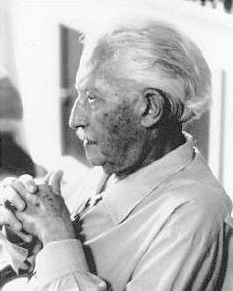
\includegraphics{figs/Erik_Erikson.jpg}
\end{center}
\end{frame}

\begin{frame}{Types of longitudinal design}
\phantomsection\label{types-of-longitudinal-design}
\begin{itemize}[<+->]
\tightlist
\item
  Trend studies
\item
  Cohort studies
\item
  Panel studies
\item
  Accelerated longitudinal designs
\end{itemize}
\end{frame}

\begin{frame}{Psychosocial theory of human development}
\phantomsection\label{psychosocial-theory-of-human-development}
Weiten (2013)
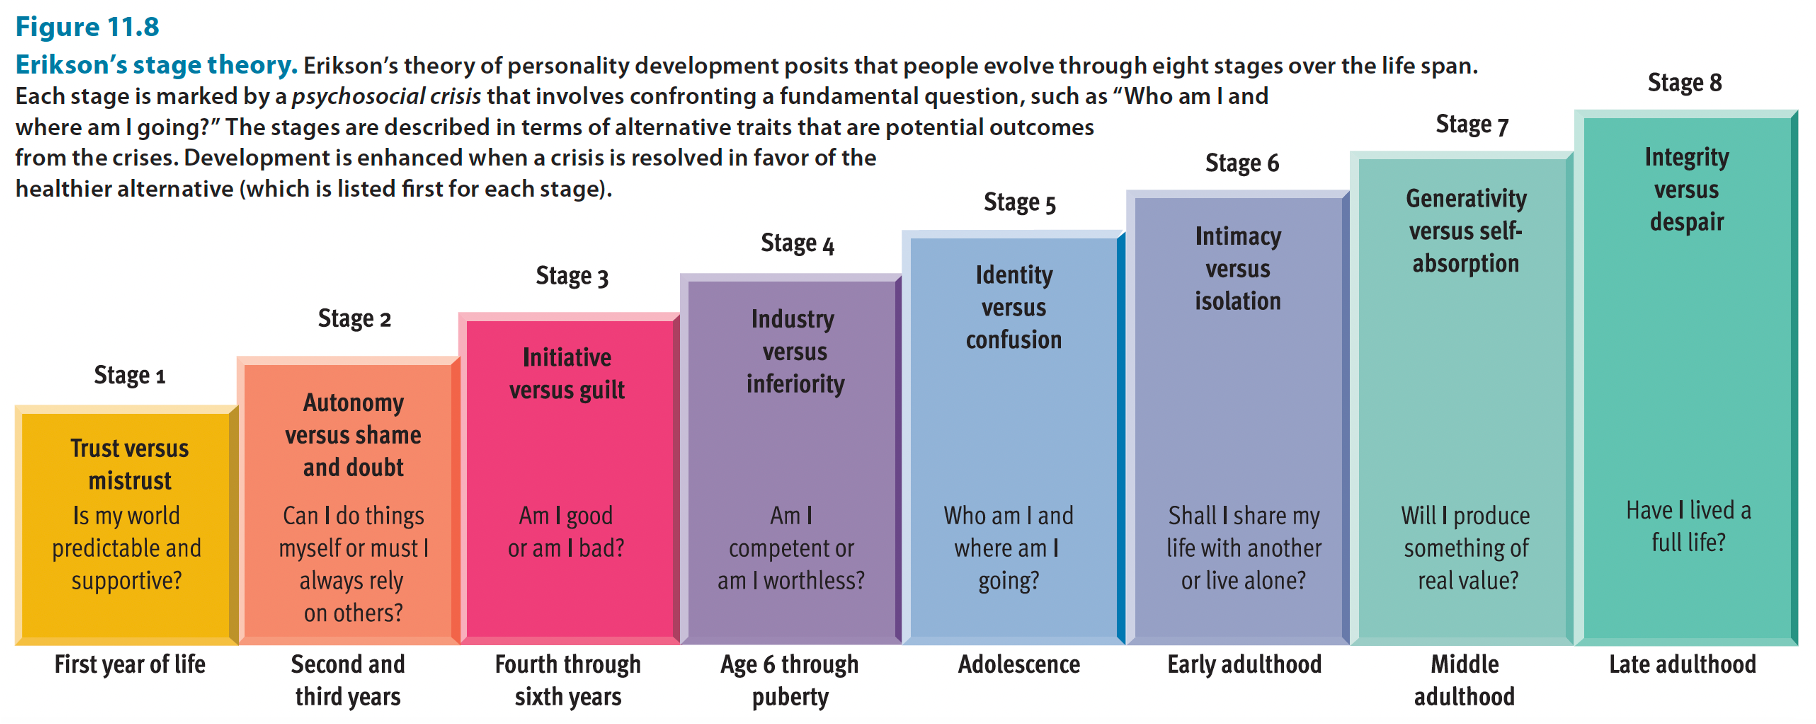
\includegraphics[width=0.9\textwidth,height=\textheight]{figs/stages.png}
\end{frame}

\begin{frame}{Marcia's identity statuses}
\phantomsection\label{marcias-identity-statuses}
Weiten (2013) 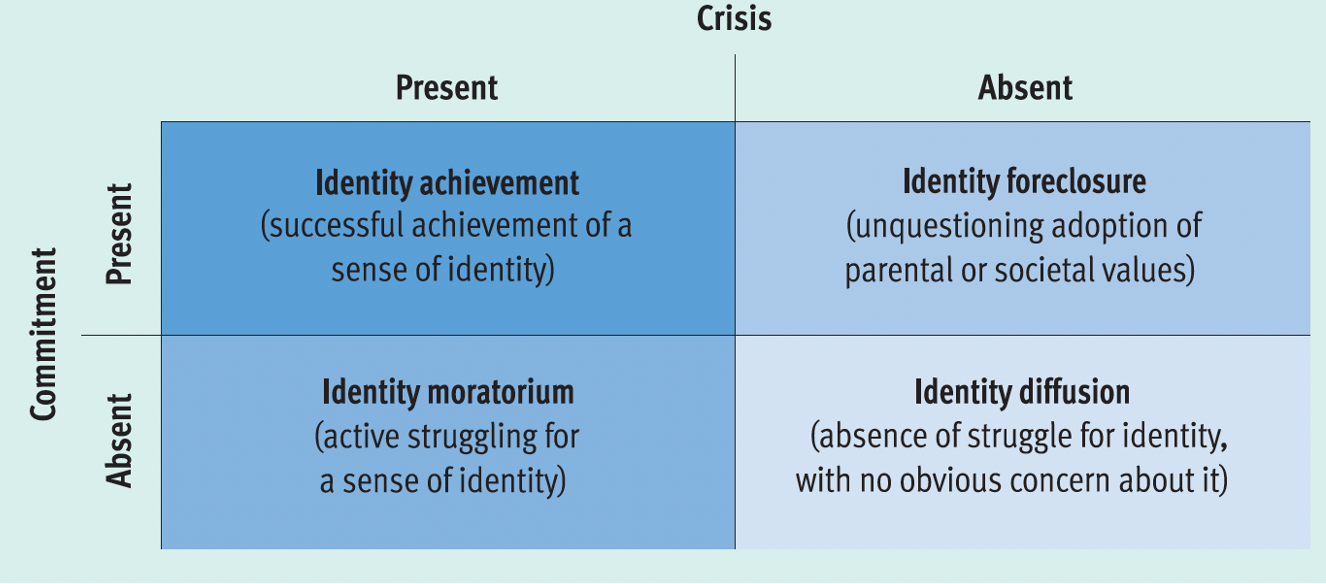
\includegraphics{figs/marcia.png} Identity achievement is
associated with higher self-esteem, conscientiousness, security,
achievement motivation, and capacity for intimacy (Kroger 2006).
\end{frame}

\section{Negative consequences}\label{negative-consequences}

\begin{frame}{Trend studies}
\phantomsection\label{trend-studies}
\begin{itemize}[<+->]
\tightlist
\item
  Trend studies, also known as time-trend studies, involve studying
  changes in a \textbf{single variable or phenomenon across different
  time points}. In trend studies, researchers collect data from
  different cross-sectional samples at various time intervals. The focus
  is on observing how the variable of interest changes over time within
  each sample, without necessarily tracking the same individuals across
  time.
\item
  Example: Tracking changes in cognitive abilities in a cohort of aging
  adults
\end{itemize}
\end{frame}

\begin{frame}{Cohort Studies}
\phantomsection\label{cohort-studies}
\begin{itemize}[<+->]
\tightlist
\item
  Cohort studies involve tracking \textbf{specific groups (cohorts)} of
  individuals over time. Cohorts are usually defined by a shared
  characteristic, such as birth year or life experience. Researchers
  collect data from the same group of individuals at multiple time
  points to study changes and developments within that specific cohort.
  This design allows for the examination of cohort-specific effects and
  trends.
\item
  Example: Comparing social attitudes in different generations
\end{itemize}
\end{frame}

\begin{frame}{Panel Studies}
\phantomsection\label{panel-studies}
\begin{itemize}[<+->]
\tightlist
\item
  Panel studies involve collecting data from the \textbf{same
  individuals} (the panel) at multiple time points. The goal is to track
  individual trajectories and changes over time. Panel studies require
  the same participants to be measured on the same variables repeatedly,
  making them well-suited for examining within-person variability and
  changes within specific individuals over time.
\item
  Example: Tracking academic performance in a group of students from
  childhood to adulthood
\end{itemize}
\end{frame}

\begin{frame}{Accelerated longitudinal design}
\phantomsection\label{accelerated-longitudinal-design}
\begin{itemize}[<+->]
\tightlist
\item
  Accelerated longitudinal designs involve \textbf{intensive data
  collection over a shorter period} compared to traditional longitudinal
  studies. This design is particularly useful when researchers are
  interested in studying rapid changes or development within a
  relatively compressed timeframe. Accelerated designs can involve
  repeated measurements over weeks or months, capturing significant
  changes in a short span.
\item
  Example: Studying language acquisition in children over a few months
\end{itemize}
\end{frame}

\begin{frame}
\textbf{Have you been in a condition that people don't believe that you
are a New Zealander?}
\end{frame}

\section{Identity denial}\label{identity-denial}

\begin{frame}{Identity denial}
\phantomsection\label{identity-denial-1}
\begin{itemize}[<+->]
\tightlist
\item
  Where are you \emph{really} from?: Asian Americans and identity denial
  (Cheryan and Monin 2005)
\item
  Leads to poor psychological health and wellbeing, such as depressive
  symptoms and stress (Albuja, Sanchez, and Gaither 2019)
\end{itemize}
\end{frame}

\begin{frame}
\textbf{Do you think our youth have an identity problem?}
\end{frame}

\section{Solutions}\label{solutions}

\begin{frame}
\begin{itemize}[<+->]
\tightlist
\item
  Individually: coping, awareness, standing up, promoting positive
  intergroup contact, building bridges
\item
  As a group: nurture a strong supportive social network
\item
  But remember that this should not be exclusive!
\end{itemize}
\end{frame}

\begin{frame}{Key differences}
\phantomsection\label{key-differences}
\begin{enumerate}[<+->]
\item
  \textbf{Focus and Purpose}: Trend studies focus on tracking changes in
  a single variable across different samples over time, while cohort
  studies focus on specific birth cohorts or groups, panel studies track
  the same individuals, and accelerated designs focus on capturing rapid
  changes.
\item
  \textbf{Sampling}: Trend studies involve different cross-sectional
  samples at each time point, cohort studies follow specific groups,
  panel studies involve the same individuals, and accelerated designs
  may involve a focused sample over a short period.
\end{enumerate}
\end{frame}

\begin{frame}{Key differences}
\phantomsection\label{key-differences-1}
\begin{enumerate}[<+->]
\setcounter{enumi}{2}
\item
  \textbf{Data collection}: Trend studies collect data from different
  samples at different times, cohort studies collect data from the same
  cohort over time, panel studies repeatedly measure the same
  individuals, and accelerated designs gather intensive data in a
  shorter duration.
\item
  \textbf{Research questions}: Trend studies are good for examining
  overall trends, cohort studies are useful for cohort-specific effects,
  panel studies can explore within-person changes, and accelerated
  designs capture rapid changes or developments.
\end{enumerate}
\end{frame}

\begin{frame}{Key differences}
\phantomsection\label{key-differences-2}
\begin{enumerate}
\setcounter{enumi}{4}
\tightlist
\item
  \textbf{Benefits and challenges}: Trend studies can identify overall
  patterns but may suffer from cohort effects; cohort studies provide
  cohort-specific insights but require long-term commitment; panel
  studies allow for individual-level analysis but can be
  resource-intensive; accelerated designs capture rapid changes but may
  not capture long-term effects.
\end{enumerate}
\end{frame}

\begin{frame}{Applications of longitudinal studies}
\phantomsection\label{applications-of-longitudinal-studies}
\begin{itemize}[<+->]
\tightlist
\item
  \textbf{Developmental psychology}
\item
  Examining cognitive, social, and emotional development
\item
  Identifying risk and protective factors for developmental outcomes
\item
  \textbf{Clinical psychology}
\item
  Tracking treatment effectiveness and relapse prevention
\item
  Understanding trajectories of mental health disorders
\end{itemize}
\end{frame}

\begin{frame}{Dunedin Multidisciplinary Health and Development Study}
\phantomsection\label{dunedin-multidisciplinary-health-and-development-study}
This study has followed a cohort of 1,037 individuals born in Dunedin,
New Zealand in 1972-1973. Participants have been assessed at various
ages to understand the development of physical health, mental health,
and social behavior over their lives. The study has provided insights
into the development of mental disorders, addiction, and antisocial
behavior.

\url{https://dunedinstudy.otago.ac.nz}
\end{frame}

\begin{frame}{The New Zealand Attitudes and Values Study (NZAVS)}
\phantomsection\label{the-new-zealand-attitudes-and-values-study-nzavs}
The New Zealand Attitudes and Values Study is a long-term research
project that began in 2009 by Prof \href{}{Chris Sibley} (The University
of Auckland). It focuses on investigating the attitudes, values, and
beliefs of New Zealanders over time. The study aims to provide a
comprehensive understanding of how various factors, including
demographics, experiences, and historical context, shape individuals'
opinions and behaviours.
\end{frame}

\begin{frame}
\begin{enumerate}
\item
  Muslims with the strongest ties to their community as measured by
  service attendance and prayer are buffered most from anti-Muslim
  prejudice.
\item
  Muslims experience greater challenges to employment and health than
  matched members of other religious groups.
\item
  Subjective well-being, the meaning of life, and psychological distress
  are similar among Muslims and matched members of religious groups from
  the buffering of religious community-making.
\end{enumerate}
\end{frame}

\begin{frame}
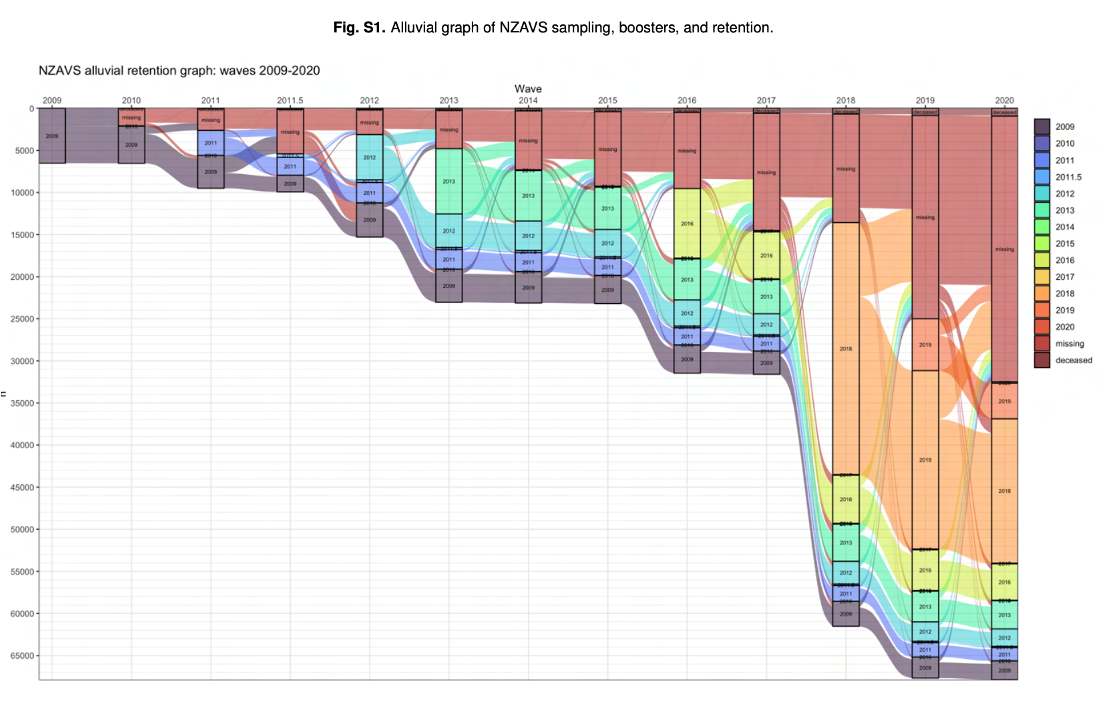
\includegraphics{figs/alluvial.png}
\end{frame}

\begin{frame}
\begin{figure}

\begin{minipage}{\linewidth}
\begin{center}

\includegraphics[width=0.6\textwidth,height=\textheight]{figs/mds.png}
\end{center}
\end{minipage}%
\newline
\begin{minipage}{\linewidth}

\includegraphics{figs/sponsors.png}\end{minipage}%

\end{figure}%
\end{frame}

\begin{frame}{NZAVS Key Features}
\phantomsection\label{nzavs-key-features}
\begin{itemize}[<+->]
\tightlist
\item
  Longitudinal Nature: The NZAVS follows a large and diverse sample of
  New Zealanders across different age groups over an extended period.
  This longitudinal design enables researchers to track changes in
  attitudes and values across generations and identify trends and shifts
  over time.
\item
  Wide Range of Topics: The study covers a broad range of topics,
  including social, political, environmental, and cultural attitudes. It
  delves into issues such as discrimination, social cohesion,
  well-being, environmental concerns, political participation, and
  national identity.
\item
  Cohort Comparison: By comparing responses from different cohorts of
  participants (e.g., different age groups), the NZAVS can highlight
  generational shifts in attitudes and values. This approach provides
  insights into how social and historical changes impact people's
  worldviews.
\end{itemize}

\begin{longtable}[]{@{}
  >{\raggedright\arraybackslash}p{(\columnwidth - 0\tabcolsep) * \real{1.0000}}@{}}
\toprule\noalign{}
\endhead
::: incremental - Data Collection Methods: The NZAVS collects data
through online or printed surveys. The surveys include both established
measures and new items designed to capture emerging issues and trends. -
Public Engagement: The study emphasizes public engagement and
transparency. Researchers share findings with the public and
policymakers, contributing to informed discussions and evidence-based
decision-making. - Impact on Policy and Society: The insights gained
from the NZAVS have the potential to inform social policies, educational
initiatives, and public discourse in New Zealand. The study's findings
can help anticipate societal changes and design interventions that
address emerging challenges. - Treatment: Treatments can happen -- but
mostly in the form of natural or man-made events (e.g., changes in the
government, some government policies/legislations, Covid-19,
earthquakes, floods, massacres). \\
::: \\
\#\# Examples of Research Questions Addressed by NZAVS \\
::: incremental 1. How have attitudes toward multiculturalism and
diversity changed over different generations? 2. What are the factors
influencing environmental attitudes and behaviors among New Zealanders?
3. How do perceptions of social inequality vary across age groups and
socioeconomic backgrounds? 4. What are the predictors of political
engagement and civic participation in New Zealand? 5. How has the
perception of national identity evolved in response to changing societal
norms and events? 6. A current NZAVS project looking at diversity and
flourishing within Muslims in NZ:
https://usman-afzali.github.io/muslim-diversity/ \\
::: \\
\# Muslim Diversity Study (MDS) \\
\#\# Important NZAVS links \\
Homepage: https://osf.io/75snb/wiki/home/ Current study group:
https://osf.io/75snb/wiki/Research\%20Group/ Publications:
https://osf.io/75snb/wiki/Publications/ \\
\#\# Aims \\
::: incremental - Increase Muslim community \textbf{representation} in
research - Increase \textbf{research opportunities} for the Muslim
community - \textbf{Share findings} back with the community members,
leadership, and government. ::: \\
\#\# FAQ's \\
::: incremental \\
- Are my responses confidential? - Can my responses be linked back to
me? - I don't like some of the questions. Is it required to answer all
questions? - How does it help Muslim community in the long run? - How
can you participate? ::: \\
\#\# MDS Team Christchurch \\
- Marzia Ehsani - Zahra Haidary - Khadija Jasim - Sarah Quader \\
\#\# MDS Auckland Team \\
- Omer Anwarzada - Ayyan Ali - Asem Arif - Weaam Bassiouni - Aqsa Butt -
Dr Iman Hussain - Abduallah Kalantan - Noor Najm \\
\#\# MDS Hamilton Team \\
- Sana Nisar Ahmad - Dr Hala Burhoum - Yasir Saifudeen \\
\#\# MDS Palmerston North Team \\
- Mashal Khan \\
\#\# MDS Wellington Team \\
- Tuba Azeem - Parus Khoso - Hawwa Niyaz - Hussain Raissi \\
\#\# MDS Dunedin Team \\
- Dr Farah Shawkat - Dr Mai Tamimi \\
\#\# MDS Media and Admin Team \\
- Jamila Badis - Noor Najm \\
\#\# MDS Core Team \\
::: \{layout=``{[}{[}40,-20,40{]}, {[}-30, 40, -30{]},
{[}40,-20,40{]}{]}''\}
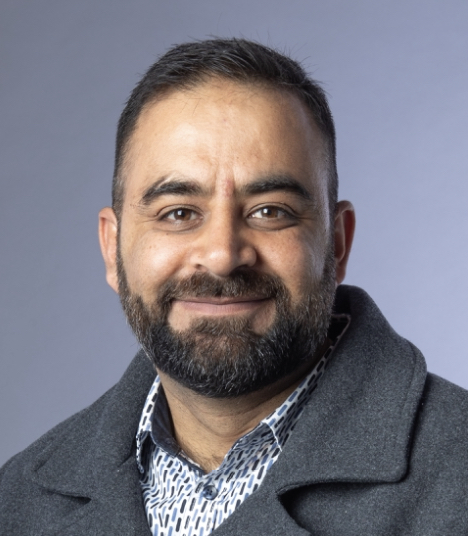
\includegraphics[width=0.9in,height=\textheight]{figs/usman-a.jpeg} \\
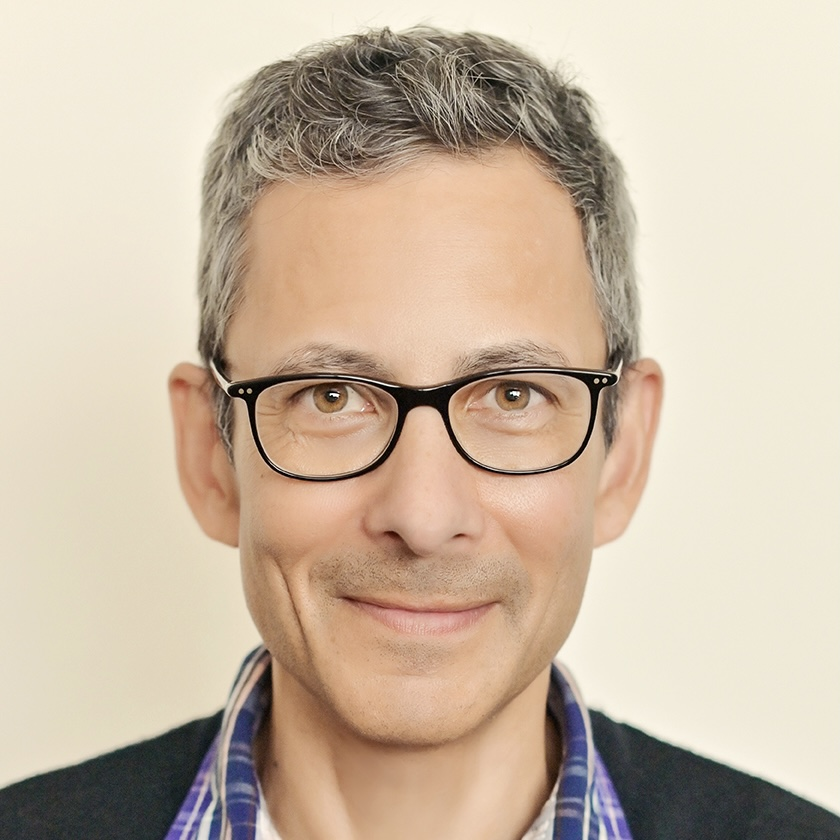
\includegraphics[width=0.9in,height=\textheight]{figs/joe-b.jpg} \\

\includegraphics[width=0.9in,height=\textheight]{figs/chris-s.png} \\
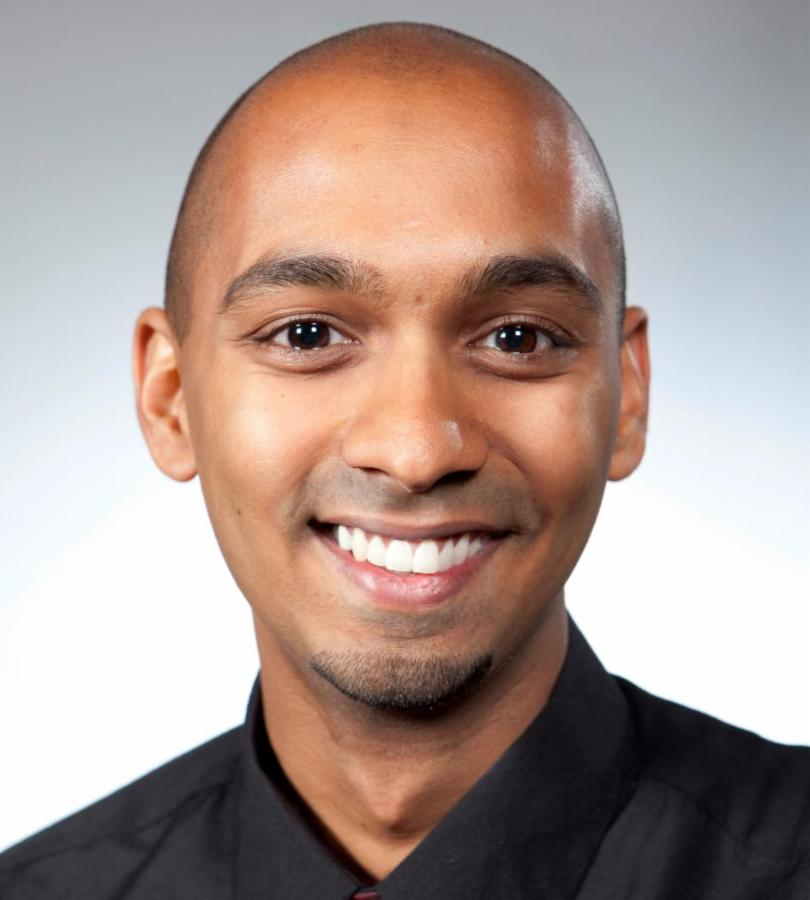
\includegraphics[width=0.9in,height=\textheight]{figs/kumar-y.jpg} \\

\includegraphics[width=0.9in,height=\textheight]{figs/aarif-r.jpeg}
::: \\
\bottomrule\noalign{}
\end{longtable}

\begin{itemize}
\tightlist
\item
  20+ Research Assistants
\item
  Numerous research collaborators
\item
  Muslim Reference Group
\end{itemize}
\end{frame}

\begin{frame}{Talks in the past}
\phantomsection\label{talks-in-the-past}

\includegraphics[width=0.4\textwidth,height=\textheight]{figs/care-lecture.png}


\includegraphics[width=0.4\textwidth,height=\textheight]{figs/uc-lecture.png}
\end{frame}

\begin{frame}{To find out more}
\phantomsection\label{to-find-out-more}

\includegraphics[width=0.5\textwidth,height=\textheight]{figs/mds-uc-banner.png}

\url{https://linktr.ee/muslimdiversity}
\end{frame}

\begin{frame}{Or use this QR code}
\phantomsection\label{or-use-this-qr-code}

\includegraphics[width=0.5\textwidth,height=\textheight]{figs/mds-qr.png}
\end{frame}

\begin{frame}{Thank you}
\phantomsection\label{thank-you}
\begin{itemize}
\tightlist
\item
  UCMUSA
\item
  Christchurch MDS Team
\item
  Asturlab Cultural Centre
\end{itemize}
\end{frame}

\begin{frame}
\textbf{Patai?}

\textbf{Ka Kite}
\end{frame}

\begin{frame}{References}
\phantomsection\label{references}
\phantomsection\label{refs}
\begin{CSLReferences}{1}{0}
\bibitem[\citeproctext]{ref-albuja2019identity}
Albuja, Analia F, Diana T Sanchez, and Sarah E Gaither. 2019.
{``Identity Denied: Comparing American or White Identity Denial and
Psychological Health Outcomes Among Bicultural and Biracial People.''}
\emph{Personality and Social Psychology Bulletin} 45 (3): 416--30.

\bibitem[\citeproctext]{ref-bosson2006}
Bosson, JENNIFER K., AMBER B. JOHNSON, KATE NIEDERHOFFER, and WILLIAM B.
SWANN. 2006. {``Interpersonal Chemistry Through Negativity: Bonding by
Sharing Negative Attitudes about Others.''} \emph{Personal
Relationships} 13 (2): 135--50.
\url{https://doi.org/10.1111/j.1475-6811.2006.00109.x}.

\bibitem[\citeproctext]{ref-cheryan2005you}
Cheryan, Sapna, and Benoı̂t Monin. 2005. {``Where Are You Really from?:
Asian Americans and Identity Denial.''} \emph{Journal of Personality and
Social Psychology} 89 (5): 717.

\bibitem[\citeproctext]{ref-fein1997a}
Fein, Steven, and Steven J. Spencer. 1997. {``Prejudice as Self-Image
Maintenance: Affirming the Self Through Derogating Others.''}
\emph{Journal of Personality and Social Psychology} 73 (1): 31--44.
\url{https://doi.org/10.1037/0022-3514.73.1.31}.

\bibitem[\citeproctext]{ref-kroger2006identity}
Kroger, Jane. 2006. {``Identity Development During Adolescence.''}
\emph{Blackwell Handbook of Adolescence}, 205--26.

\bibitem[\citeproctext]{ref-weaver2011}
Weaver, Jonathan R., and Jennifer K. Bosson. 2011. {``I Feel Like I Know
You: Sharing Negative Attitudes of Others Promotes Feelings of
Familiarity.''} \emph{Personality and Social Psychology Bulletin} 37
(4): 481--91. \url{https://doi.org/10.1177/0146167211398364}.

\end{CSLReferences}
\end{frame}



\end{document}
